\documentclass[tikz]{standalone}

\usepackage[greek,english]{babel}

\usepackage{pgfplots}
\usetikzlibrary{decorations.pathreplacing}

\pagecolor{white}

\begin{document}
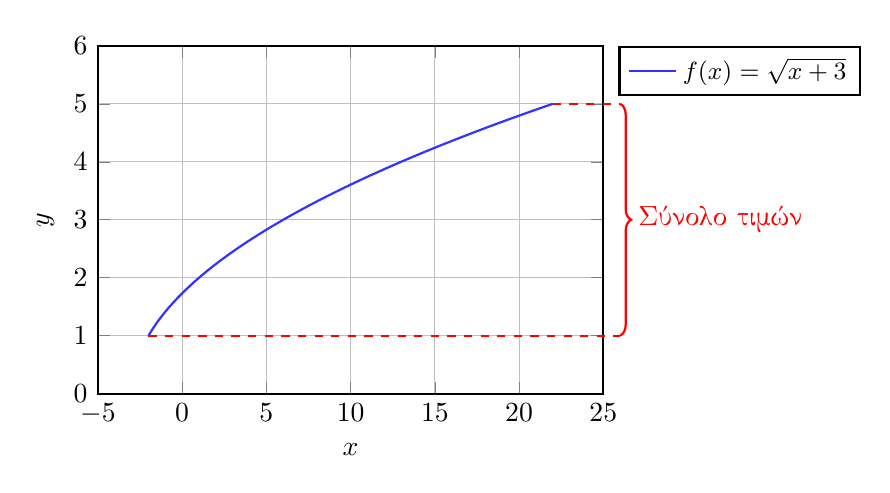
\begin{tikzpicture}
\begin{axis}[
    width=8cm,
    height=6cm,
    domain=-5:20, 
    xmin=-5,
    xmax=25,
    ymin=0,
    ymax=6,
    thick,
    ytick={0,1,2,3,4,5,6},
    xtick={-5,0,5,10,15,20,25},
    legend pos=outer north east,
    mark size=1.5pt,
    xlabel={$x$},
    ylabel={$y$},
    legend cell align={left},
    clip=false, % To avoid cropping the label.
    grid]

\draw [decorate,decoration={brace,amplitude=4pt},red]
      (axis cs:26,5) -- (axis cs:26,1) node [midway,right,xshift=.1cm] {\textgreek{Σύνολο τιμών}}; 
\draw [dashed,red] (axis cs:-2,1) -- (axis cs:26,1);
\draw [dashed,red] (axis cs:22,5) -- (axis cs:26,5);

\addplot[red, domain=-2:22,restrict y to domain=0:8, samples=100, blue!80!white]  {(x+3)^0.5};

\addlegendentry{\small $f(x) = \sqrt{x+3}$ }


\end{axis}
\end{tikzpicture}
\end{document}

